\chapter{Benchmark, Fine-Tuning, and Budget Results}
\label{chap:benchmark-results}

\section{Final-answer benchmark}

The lexical benchmark establishes the outcome pattern before intermediate states are considered. On the harder MuSiQue subset, the frozen SAS achieves final normalised accuracy of 0.560 at the 1,000-token budget and 0.525 at 2,000. Debate is the strongest MAS in this condition, at 0.510 and 0.535 respectively. Sequential is substantially lower, at 0.335 and 0.340. Fine-tuning does not reverse the broad ranking: at 1,000 tokens the \texttt{v3b} SAS scores 0.545, Debate 0.505, and Sequential 0.380.

\begin{table}[htbp]
  \centering
  \caption[MuSiQue final lexical accuracy]{MuSiQue final normalised lexical accuracy by model, architecture, and thinking-token budget ($n=200$ per cell).}
  \label{tab:musique-lexical}
  \begin{tabular}{@{}llrr@{}}
    \toprule
    Model & System & 1,000 & 2,000 \\
    \midrule
    Frozen & SAS & \textbf{0.560} & 0.525 \\
           & Debate & 0.510 & \textbf{0.535} \\
           & Ensemble & 0.520 & 0.505 \\
           & Parallel Roles & 0.425 & 0.390 \\
           & Sequential & 0.335 & 0.340 \\
           & Subtask Parallel & 0.425 & 0.425 \\
    \addlinespace
    v3b & SAS & \textbf{0.545} & \textbf{0.530} \\
        & Debate & 0.505 & \textbf{0.530} \\
        & Ensemble & 0.515 & 0.510 \\
        & Parallel Roles & 0.415 & 0.445 \\
        & Sequential & 0.380 & 0.340 \\
        & Subtask Parallel & 0.410 & 0.390 \\
    \bottomrule
  \end{tabular}
\end{table}

On 2WikiMultiHopQA, absolute performance is much higher. In the frozen condition, Debate reaches 0.935 and 0.930 at the two budgets, compared with SAS at 0.860 and 0.845. This is an important counterexample to any universal statement that a single agent always wins: an MAS can outperform the SAS on a particular dataset and condition. The dissertation's claim is narrower. Multi-agent decomposition often increases candidate availability, but that gain is inconsistent and can be lost at later coordination stages. Relative performance depends on dataset difficulty, model variant, architecture, and budget.

\subsection{Fine-tuning as an attempted intervention}

The \texttt{v3b} comparison is treated as an attempted intervention after the initial frozen-model benchmark rather than as a separate model family. On MuSiQue, its changes are mixed. At 1,000 tokens, SAS changes from 0.560 to 0.545, Debate from 0.510 to 0.505, and Sequential from 0.335 to 0.380. At 2,000 tokens, SAS changes from 0.525 to 0.530, Debate from 0.535 to 0.530, and Sequential remains at 0.340. These cells do not show a consistent reversal of the SAS--MAS pattern. Because \texttt{v3b} was trained primarily on single-agent-style data, this result does not test whether architecture-conditioned training for planners, critics, or aggregators would succeed.

The final-answer results establish what happened but cannot determine whether an architecture failed to discover the reference answer or failed to preserve and select an answer that had already appeared. That mechanism is examined only after the budget intervention is reported.

\section{Budget effects}

The matched budget analysis provides no evidence that doubling the nominal thinking allowance improves aggregate MAS outcomes. Across 3,997 resolved discovery pairs, machine-screened semantic discovery falls from 0.8419 at 1,000 tokens to 0.8284 at 2,000. There are 138 wrong-to-correct changes but 192 correct-to-wrong changes; the exact McNemar $p$-value is 0.0035. Across all 4,000 final pairs, machine-screened semantic final accuracy falls from 0.7408 to 0.7282, with 241 wrong-to-correct and 291 correct-to-wrong changes ($p=0.0335$). Mean wall time rises by 4.83 seconds and mean realised thinking increases by approximately 495 tokens.

\begin{figure}[htbp]
  \centering
  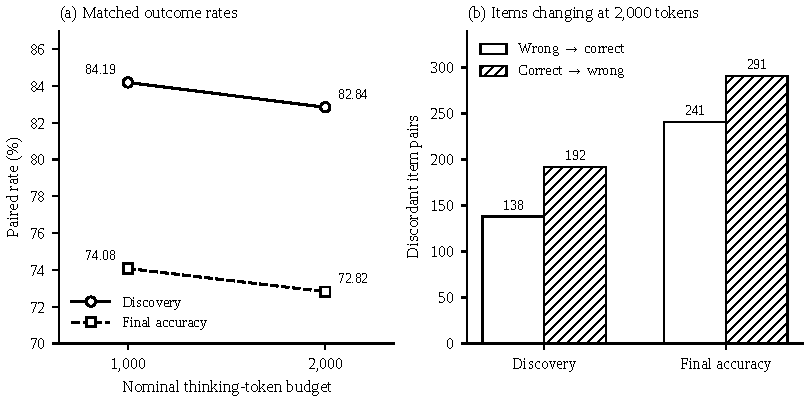
\includegraphics[width=0.92\textwidth]{figures/budget_tradeoff.pdf}
  \caption[Matched budget outcomes]{Matched aggregate outcomes at 1,000 and 2,000 nominal thinking tokens. The larger budget increases mean wall time while reducing machine-screened discovery and final semantic accuracy.}
  \label{fig:budget}
\end{figure}

The architecture-level results are heterogeneous. Debate final accuracy changes from 0.8113 to 0.7850 ($p=0.106$), Ensemble from 0.7725 to 0.7500 ($p=0.066$), Parallel Roles from 0.7425 to 0.7412 ($p=1.000$), Sequential from 0.6650 to 0.6538 ($p=0.426$), and Subtask Parallel from 0.7125 to 0.7113 ($p=1.000$). None of these individual final-accuracy comparisons reaches the conventional 0.05 level. The aggregate decline is produced by many small, mostly non-improving changes across cells rather than one architecture collapsing.

Latency increases in every system. Debate mean wall time rises from 15.38 to 22.92 seconds; Ensemble from 7.57 to 10.88; Parallel Roles from 9.94 to 14.79; Sequential from 17.89 to 22.58; and Subtask Parallel from 11.66 to 15.40. Parallel systems have shorter critical paths, but this should not be confused with lower total device work.

\section{Chapter summary}

The outcome experiments establish three constraints on the explanation developed in the following chapters. First, SAS is not universally superior: the ordering changes by dataset and architecture. Second, the completed fine-tuning intervention does not consistently remove the observed gaps. Third, a larger nominal token cap increases resource use without improving aggregate semantic outcomes. These findings motivate the next question: whether the systems fail because they do not discover a correct answer or because later components do not preserve it. \Cref{chap:machine-results} addresses that question using the full-trace machine screen.
